\begin{ZhChapter}

\chapter{相關技術與背景}

\section{藍牙低功耗技術(Bluetooth Low Energy, BLE)}

藍牙技術聯盟(Bluetooth Special Interest Group)在2010年6月發布了可以短距離數據交換和低功耗的藍芽低功耗技術(Bluetooth Low Energy, BLE)。而藍芽低功耗技術被發布後,就被物聯網(IoT)廣泛的應用,包括了家庭娛樂、醫療保健、運動健身、安防以及信標等領域。

藍牙低功耗技術(Bluetooth Low Energy, BLE)是一種功耗極低的技術,這一個技術讓裝置在大部分的時間都在休眠模式,只有在需要使用該裝置時,才會快速喚醒進行工作,這讓BLE裝置僅需要一顆鈕扣電池就可以運作數月甚至數年之久,這讓BLE生產成本更低,且保留了傳統藍芽(Classic Bluetooth)類似的通訊範圍,且一樣相容於手機、平板電腦等設備。

BLE運作在2.4G的ISM頻段,利用FDMA,將2402MHz~2480MHz分成40個Channel,又將這些Channel又分成兩種傳輸模式,廣播模式(Advertising Mode)及連線模式(Connection-Oriented Mode),其中廣播模式使用了Channel 37、Channel 38、Channel 39,工作頻率分別是2403MHz、2426MHz、2480MHz,剩餘的37個Channel為連接模式使用,如圖(2.1)所示。

\begin{figure*}[htbp]
    \centering
    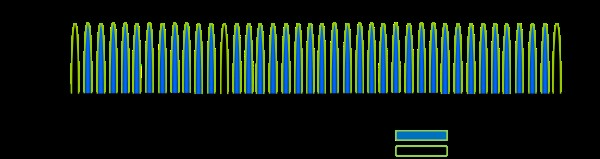
\includegraphics[width = 1\textwidth]{image/廣播頻道與資料頻道示意圖.jpg}
    \caption{廣播頻道與資料頻道示意圖\cite{microchip2023}}
    \label{fig: 廣播頻道與資料頻道示意圖}
\end{figure*}

廣播模式和連接模式的運作機制由 BLE 的控制層(Controller Layer)狀態機管理,包括Standby(等待)、Advertising(廣播)、Scanning(掃描)、Initiating(初始化)、Connection(連接)五種狀態 ,如圖(3)所示。

\begin{figure*}[htbp]
    \centering
    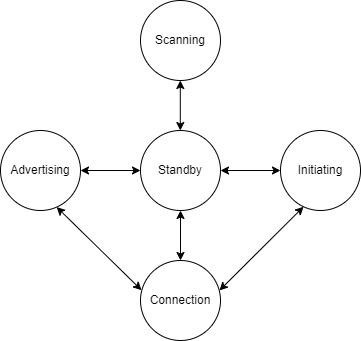
\includegraphics[width = 1\textwidth]{image/controller layer 狀態機示意圖.jpg}
    \caption{Controller layer 狀態機示意圖\cite{microchip2023}}
    \label{fig: 廣播頻道與資料頻道示意圖}
\end{figure*}


\subsection{模型說明(小標)}

說明說明說明說明,說明說明說明說明說明說明說明說明說明說明說明說明,說明說明說明說明說明說明說明說明。

\begin{figure*}[htbp]
    \centering
    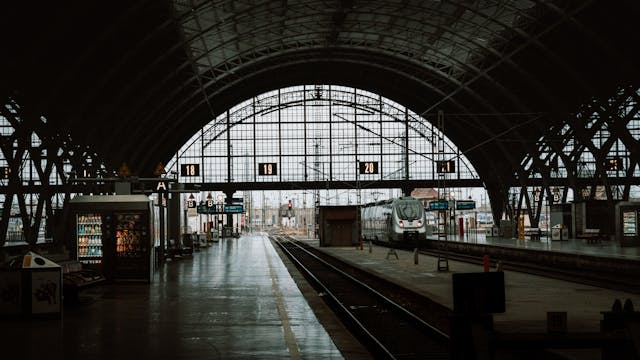
\includegraphics[width = 0.5\textwidth]{image/image.jpeg}
    \caption{Cool train station}
    \label{fig: image}
\end{figure*}

\end{ZhChapter}